\subsection{Diseño de la cimentación}
Se presentaran las consideraciones para el dimensionamiento de la cimentación, control de presiones y el cálculo del refuerzo con las verificaciones necesarias en concreto armado.\\
Se asumen dos hipótesis básicas:
\begin{enumerate}
    \item El suelo es homogéneo, elástico y aislado del suelo circundante.
    \item Considerar la flexibilidad de la Cimentación y del suelo.
\end{enumerate}

\subsubsection{Modelamiento}
El modelo matemático simple que se usa en la practica consiste en incluir la flexibilidad del suelo a través de módulos de subrasante, el modelo más conocido es la solución de Winkler.\\
Es un modelo aproximado que se propuso en 1867, el cual sirve para resolver fundaciones sobre medios elásticos. Este método considera el suelo como un lecho de resortes. La presión de contacto queda definida por el producto de la rigidez elástica del resorte y el asentamiento que se ha producido en él debido a las cargas que actúan.\\

\begin{figure}[h!]
    \centering
    \caption{Modelamiento de la cimentación}
    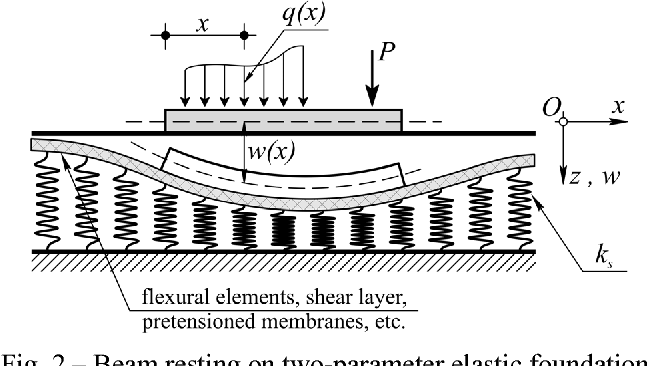
\includegraphics[trim={0 0.5cm 0 0},clip,scale=0.6]{IMAGENES/safe2.png}
    %\caption*{\small Fuente: \it \cite{empuje}}
    \label{atrans}
\end{figure} 
\newpage
En su tesis de maestría el ingeniero Nelson Morrison recopila varios estudios anteriormente realizados que relacionan directamente el módulo de subrasante con la capacidad admisible del suelo, el cual es válido para un área y NO necesita ser modificado a las dimensiones de la cimentación.

\begin{figure}[h!]
    \centering
    \caption{Coeficientes de Winkler}
    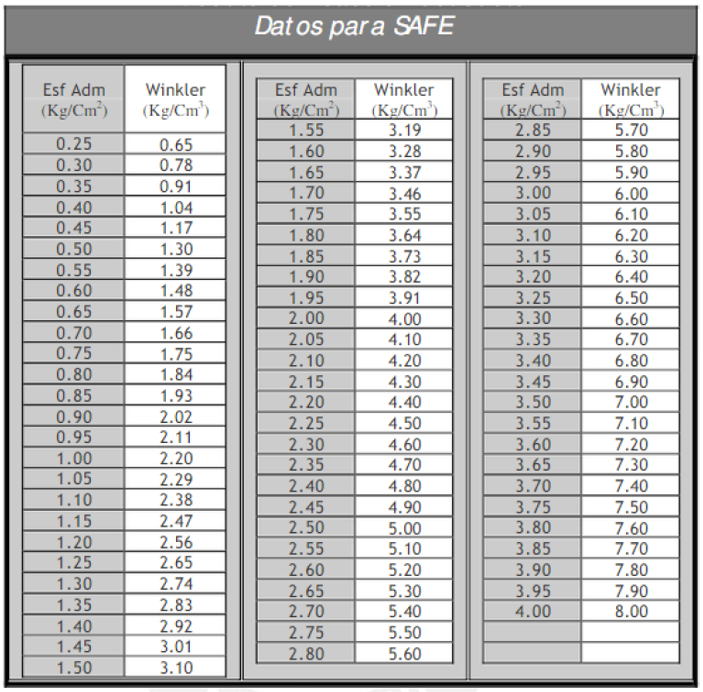
\includegraphics[scale=1]{IMAGENES/safe3.PNG}
    %\caption*{\small Fuente: \it \cite{empuje}}
    \label{atrans}
\end{figure} 

Cabe resaltar que para el diseño de fundaciones SAFE usa el Modelo de Winkler , el cual se resuelve a través del método de los elementos finitos FEM, usando elementos línea, áreas y resorte.\\
Structural Analysis by Finite Elements (SAFE), es un software creado por la empresa Computers and Structures, Inc. (CSI) , el cual sirve para diseñar sistemas de pisos ( Losas y Vigas) y Sistemas de Fundaciones.
\begin{figure}[h!]
    \centering
    \caption{SAFE}
    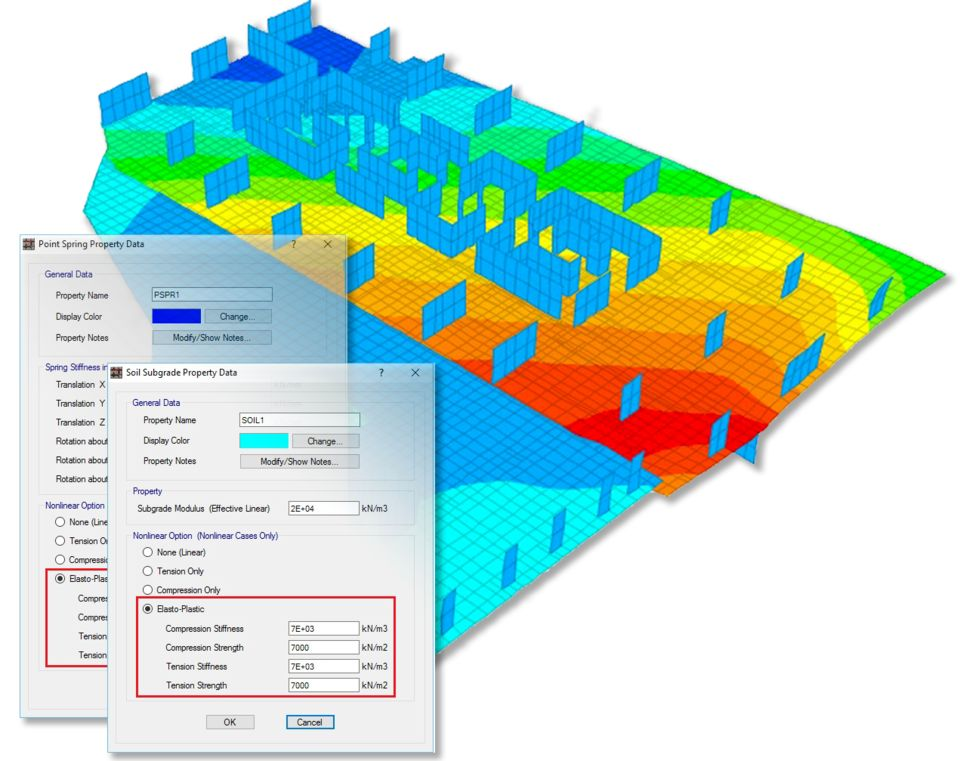
\includegraphics[scale=0.3]{IMAGENES/33.jpg}
    %\caption*{\small Fuente: \it \cite{empuje}}
    \label{atrans}
\end{figure} 

\subsubsection{Tipología de la cimentación}
Se proyectan zapatas aisladas, zapatas combinadas y plateas parciales, debido a la presencia de las edificaciones vecinas las cimentaciones resultan excéntricas en 3 lados del edificio por lo que se hace uso de vigas rígidas de cimentación para controlar los momentos producto de la excentricidad de la carga axial. Tales vigas son diseñadas solo para tomar los momentos y uniformizar las presiones en la cimentación y no es diseñada para soportar fuerzas inducidas por la presión del suelo, por lo que debe ser aislada del suelo adecuadamente.\\
El peralte de la cimentación adoptado es el requerido para las solicitaciones de corte y/o punzonamiento en la cimentación, así como para asegurar el desarrollo del refuerzo que llega de las columnas y muros.\\
En las zapatas aisladas no existe momentos que traccionen la cara superior de la zapata por lo que no es necesario colocar refuerzo superior, sin embargo en las zapatas combinadas o cuando se colocan vigas de conexión si existen momento positivo y negativo, por lo que es necesario colocar doble malla.

\subsubsection{Exportación de cargas de ETABS a SAFE}
Debido a que los resultados del análisis modal espectral son productos de una combinación se pierde el signo en las fuerzas, para un análisis racional se exporto las cargas de los modos principales en ambas direcciones escalando sus valores proporcionalmente al valor los momentos totales en la base que se generan a partir de las fueras sísmicas de diseño.

\subsubsection{Predimensionamiento}

Se dimensiono preliminarmente considerando cargas en servicio (D+L) con un 90\% de la capacidad portante para tener holgura cuando se verifica con cargas sísmicas, posteriormente estas dimensiones se corrigieron después del análisis.\\
Para las zapatas combinadas se trató de hacer coincidir el centro de gravedad de la zapata con el de las cargas para el caso de cargas gravitacionales (D+L), adicionalmente en todos los casos se dimensiono tratando de tener volados iguales en ambas direcciones para uniformizar el diseño en concreto armado.\\
Después de realizar un análisis iterativo se obtiene las áreas de cimentación mostradas en la figura  para no superar la presión admisible tanto para cargas de gravedad y sísmicas. .

\subsubsection{Control de presiones}
\begin{theo}[15.2.4 y 15.2.5 de la norma E-060:]{thm:ca1}
15.2.4 Se podrá considerar un incremento del 30\% en el valor de la presión admisible del suelo para los estados de cargas en los que intervengan cargas temporales, tales como sismo o viento.\\
15.2.5 Para determinar los esfuerzos en el suelo o las fuerzas en pilotes, las acciones sísmicas podrán reducirse al 80\% de los valores provenientes del análisis, ya que las solicitaciones sísmicas especificadas en la NTE E.030 Diseño Sismorresistente están especificadas al nivel de resistencia de la estructura.
\end{theo}
\newpage
\noindent Por lo tanto las combinaciones para el control de presiones en condiciones de servicio sera:
\begin{center}
    S1= CM + CV\\
    S2= ( CM+CV + 0.8 SX )/1.3\\
    S3= ( CM+CV - 0.8 SX )/1.3\\
    S4= ( CM+CV + 0.8 SY )/1.3\\
    S5= ( CM+CV - 0.8 SY )/1.3 
\end{center}
\noindent 
Donde:\\
CM: Carga muerta en servicio\\
CV: Carga viva en servicio\\
SX: Carga sísmica en dirección X\\
SY: Carga sísmica en dirección Y\\

\begin{figure}[h!]
    \centering
    \subfigure[Sin vigas de conexión]{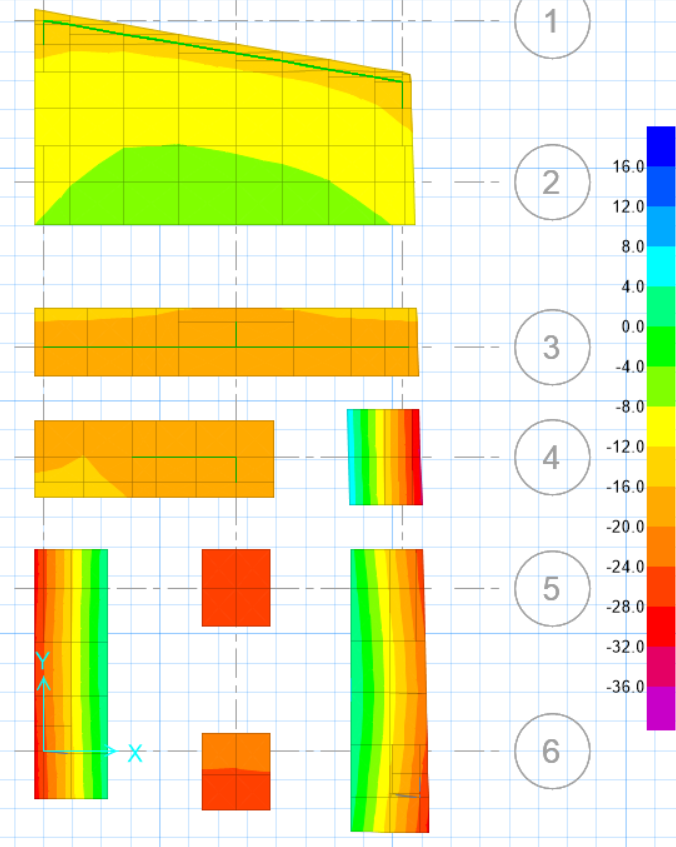
\includegraphics[width=70mm]{IMAGENES/wvc.PNG}}\hspace{10mm}
    \subfigure[Con vigas de conexión de 30x70]{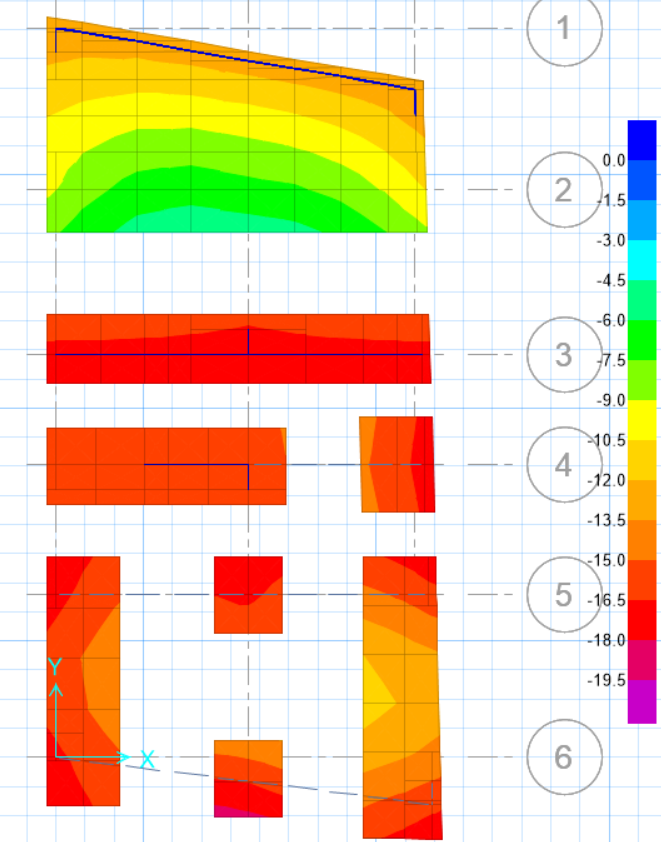
\includegraphics[width=70mm]{IMAGENES/co1.PNG}}
    \caption{Presiones para la combinación D+L }
    \label{corw}
\end{figure}
\newpage
\begin{figure}[h!]
    \centering
    \subfigure[D+L+SX]{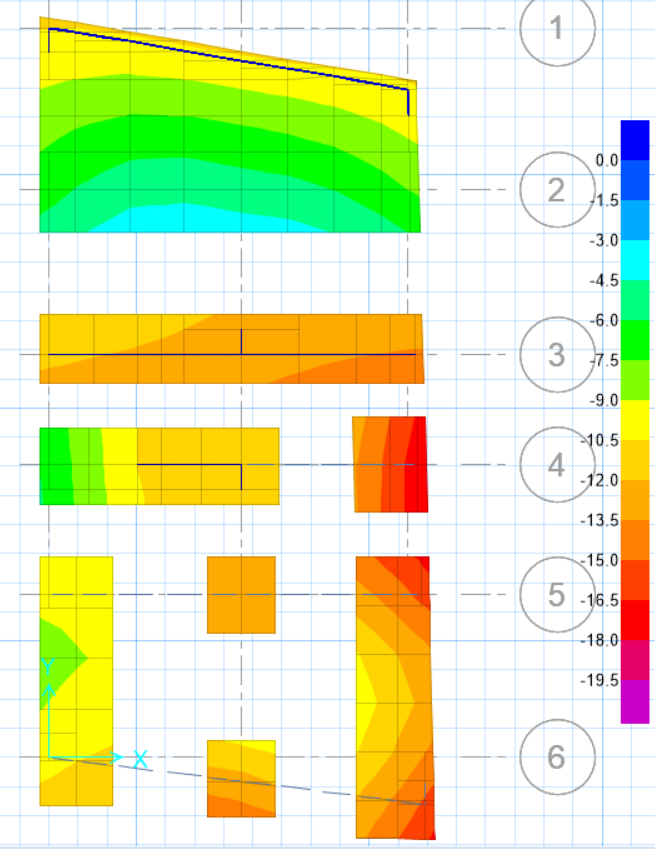
\includegraphics[width=70mm]{IMAGENES/co2.PNG}}\hspace{10mm}
    \subfigure[D+L-SX]{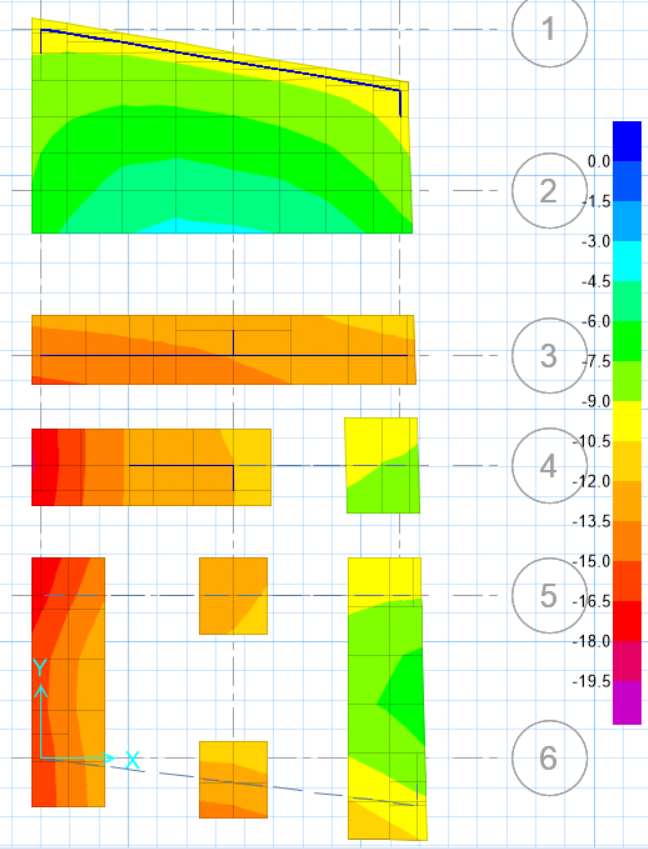
\includegraphics[width=70mm]{IMAGENES/co3.PNG}}
    \caption{Presiones para la combinación con sismo en X}
    \label{corw}
\end{figure}

\begin{figure}[h!]
    \centering
    \subfigure[D+L+SY]{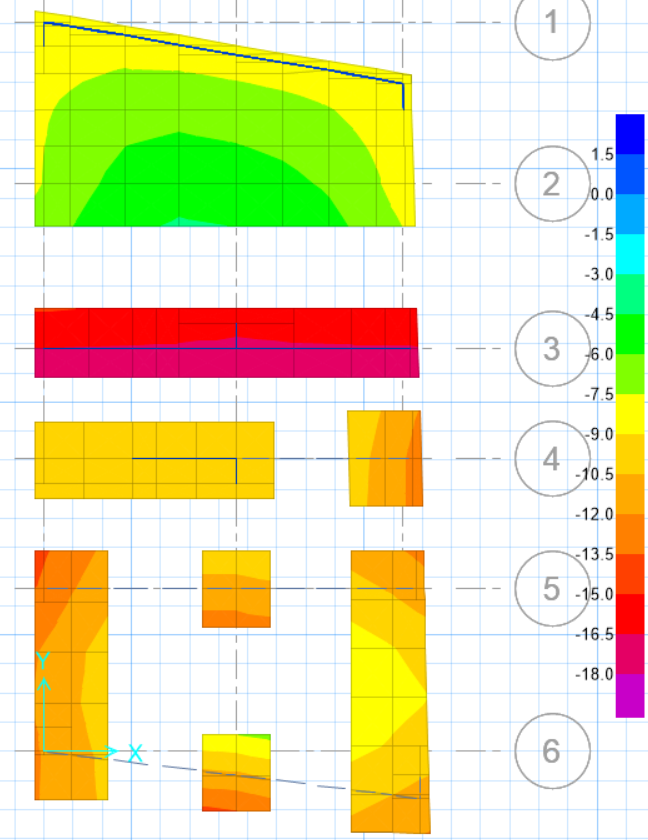
\includegraphics[width=70mm]{IMAGENES/co4.PNG}}\hspace{10mm}
    \subfigure[D+L-SY]{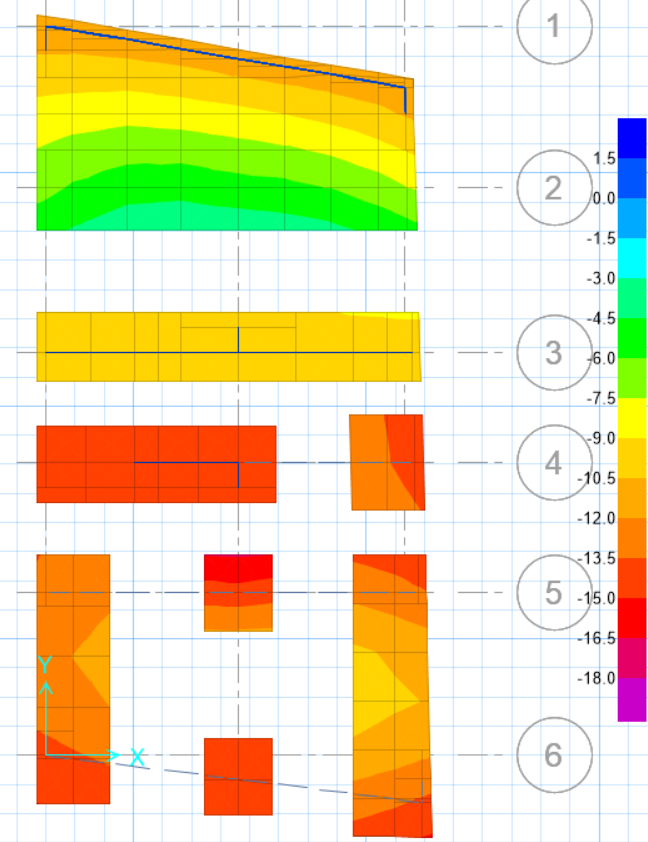
\includegraphics[width=70mm]{IMAGENES/co5.PNG}}
    \caption{Presiones para la combinación con sismo en Y}
    \label{corw}
\end{figure}
\noindent
La capacidad portante admisible del terreno a -2.8m donde se cimienta la parte frontal del edifico es de $1.82\mathrm{~kg/cm^2} $.\\
En la parte posterior a una cota de +0.50m la capacidad portante admisible del terreno es $1.42\mathrm{~kg/cm^2}$.\\
En todos los casos se cumple con la condición: $q_{u}\leq q_{n}$, siendo el caso mas critico la combinación de cargas gravitacionales dado que las cargas sísmicas se reducen considerablemente debido a lo mencionado en los artículos 15.2.4 y 15.2.5 de la \cite{E-060}.\\
Las dimensiones finales se muestran en la figura \ref{dim}:
\begin{figure}[h!]
    \centering
    \caption{Dimensiones de la cimentación}
    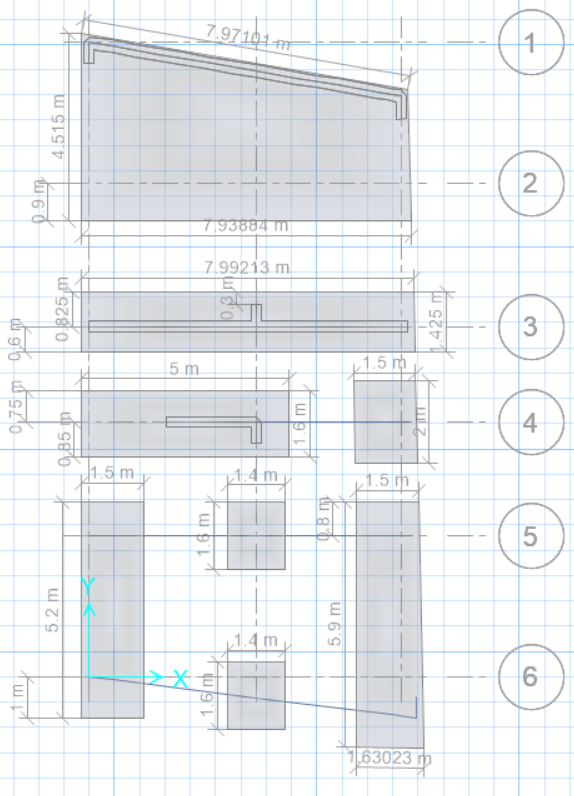
\includegraphics[scale=0.9]{IMAGENES/dim.PNG}
    %\caption*{\small Fuente: \it \cite{empuje}}
    \label{dim}
\end{figure} 

\newpage
\subsubsection{Diseño en concreto armado}
\noindent 
Según el articulo 10.5.4 la cuantía mínima en zapatas sera de 0.0018, y cuando el refuerzo se distribuya en 2 capas la cuantía mínima en la cara en tracción sera 0.0012.\\
Después de realizar el diseño en concreto armado con los requisitos mínimos de la norma se obtuvo los siguientes armados en la cimentación:
% Please add the following required packages to your document preamble:
% \usepackage{multirow}
\begin{table}[h!]
\caption{Refuerzo en cimentación}
{
\extrarowheight = 0ex
\renewcommand{\arraystretch}{1.2}
\begin{tabular}{|cc|cc|c|c|c|}
\hline
\multicolumn{2}{|c|}{\textit{\textbf{CIMENTACION}}}                       & \multicolumn{2}{c|}{\textit{\textbf{Refuerzo}}}                    & \textit{\textbf{Espesor}} & \textit{\textbf{Ancho}} & \textit{\textbf{Largo}} \\ \hline
\multicolumn{1}{|c|}{\textit{\textbf{N°}}} & \textit{\textbf{Ubicación:}} & \multicolumn{1}{c|}{\textit{\textbf{X-X}}} & \textit{\textbf{Y-Y}} & \textit{\textbf{e (cm)}}  & \textit{\textbf{B (m)}} & \textit{\textbf{L (m)}} \\ \hline
\multicolumn{1}{|c|}{\multirow{2}{*}{1}}   & Inferior                     & \multicolumn{1}{c|}{1/2"@17.5cm}           & 1/2"@17.5cm           & 55                        & \multirow{2}{*}{var}    & \multirow{2}{*}{var}    \\ \cline{2-5}
\multicolumn{1}{|c|}{}                     & Superior                     & \multicolumn{1}{c|}{5/8"@22.5cm}           & 5/8"@22.5cm           & 55                        &                         &                         \\ \hline
\multicolumn{1}{|c|}{\multirow{2}{*}{2}}   & Inferior                     & \multicolumn{1}{c|}{1/2"@17.5cm}           & 5/8"@22.5cm           & 55                        & \multirow{2}{*}{1.425}  & \multirow{2}{*}{var}    \\ \cline{2-5}
\multicolumn{1}{|c|}{}                     & Superior                     & \multicolumn{1}{c|}{1/2"@17.5cm}           & 1/2"@17.5cm           & 55                        &                         &                         \\ \hline
\multicolumn{1}{|c|}{\multirow{2}{*}{3}}   & Inferior                     & \multicolumn{1}{c|}{5/8"@22.5cm}           & 1/2"@17.5cm           & 55                        & \multirow{2}{*}{1.6}    & \multirow{2}{*}{5}      \\ \cline{2-5}
\multicolumn{1}{|c|}{}                     & Superior                     & \multicolumn{1}{c|}{5/8"@22.5cm}           & 1/2"@17.5cm           & 55                        &                         &                         \\ \hline
\multicolumn{1}{|c|}{\multirow{2}{*}{4}}   & Inferior                     & \multicolumn{1}{c|}{5/8"@22.5cm}           & 1/2"@17.5cm           & 55                        & \multirow{2}{*}{1.5}    & \multirow{2}{*}{2}      \\ \cline{2-5}
\multicolumn{1}{|c|}{}                     & Superior                     & \multicolumn{1}{c|}{1/2"@17.5cm}           & 1/2"@17.5cm           & 55                        &                         &                         \\ \hline
\multicolumn{1}{|c|}{\multirow{2}{*}{5}}   & Inferior                     & \multicolumn{1}{c|}{1/2"@17.5cm}           & 5/8"@20cm             & 60                        & \multirow{2}{*}{1.5}    & \multirow{2}{*}{5.2}    \\ \cline{2-5}
\multicolumn{1}{|c|}{}                     & Superior                     & \multicolumn{1}{c|}{1/2"@17.5cm}           & 1/2"@17.5cm           & 60                        &                         &                         \\ \hline
\multicolumn{1}{|c|}{\multirow{2}{*}{6}}   & Inferior                     & \multicolumn{1}{c|}{5/8"@20cm}             & 5/8"@20cm             & 55                        & \multirow{2}{*}{1.4}    & \multirow{2}{*}{1.6}    \\ \cline{2-5}
\multicolumn{1}{|c|}{}                     & Superior                     & \multicolumn{1}{c|}{---}                   & ---                   & 55                        &                         &                         \\ \hline
\multicolumn{1}{|c|}{\multirow{2}{*}{7}}   & Inferior                     & \multicolumn{1}{c|}{1/2"@17.5cm}           & 5/8"@20cm             & 60                        & \multirow{2}{*}{var}    & \multirow{2}{*}{5.9}    \\ \cline{2-5}
\multicolumn{1}{|c|}{}                     & Superior                     & \multicolumn{1}{c|}{1/2"@17.5cm}           & 1/2"@17.5cm           & 60                        &                         &                         \\ \hline
\end{tabular}
}
\end{table}